\chapter{様々な技}

ROOTでそこそこ格好良い図を作るには、ある程度の知識と慣れが必要になります。ここでは、いくつかのスクリプトとその出力結果を例示し、ROOTで望み通りの図を作るにはどうすれば良いかを紹介します。

\section{色関連}
\subsection{自前のカラーパレットを定義する}

ROOTでは、2次元ヒストグラムや2次元グラフの「高さ」を表現する手段として、色を用いることができます。これは第\ref{chap:Histogram}章でも説明しました。ROOTはいくつかのカラーパレット(color palette)を用意してくれていますが、それらの実用性は乏しいと言わざるを得ません。例えば図\ref{fig:multi_palette_pdf}の左上に示したような、デフォルトのカラーパレットを使っている人はほとんど見かけません。また階調数が小さめに設定されているため、滑らかな色表現には向きません。唯一よく使われているのが、以下の設定です。
\begin{lstlisting}[language=C++]
root [0] gStyle->SetPalette(1)
\end{lstlisting}
レインボーカラー(rainbow color)などと呼ばれることがあります。他にデフォルトで用意されているパレットについては、\url{http://root.cern.ch/root/html/TColor.html#TColor:SetPalette}を参照してください。

コード\ref{code:color_def}では、自分好みのカラーパレットを作る方法を示しています。原理は単純で、作りたいパレットに応じて、\texttt{TColor::CreateGradientColorTable}を呼び出すための関数を用意するだけです。いくつか例を書きましたが、原理は一緒なので関数BPalette()の解説のみをします。

\begin{NoFloat}
\lstinputlisting[language=c++,caption=\texttt{color\_def.C},label=code:color_def,numbers=left]{src/color_def.C}
\end{NoFloat}

次の4行が、実際に色の設定をする部分です。
\begin{lstlisting}[language=c++]
  Double_t r[] = {0., 0.0, 1.0, 1.0, 1.0}; 
  Double_t g[] = {0., 0.0, 0.0, 1.0, 1.0}; 
  Double_t b[] = {0., 1.0, 0.0, 0.0, 1.0}; 
  Double_t stop[] = {0., .25, .50, .75, 1.0}; 
\end{lstlisting}
最初の3行でRGB各色の輝度情報を設定します。例えば$\mathrm{R}=\mathrm{G}=\mathrm{B}=1$であれば白、$\mathrm{R}=\mathrm{G}=\mathrm{B}=0$であれば黒、$\mathrm{R}=\mathrm{G}=1$、$\mathrm{B}=0$であれば黄色といった具合です。次の行は、それらの色がヒストグラムの最小値($\equiv0$)から最大値($\equiv1$)のどこに相当するかを決めています。

グラデーションをROOTに登録する作業は、
\begin{lstlisting}[language=c++]
  Int_t index = TColor::CreateGradientColorTable(5, stop, r, g, b, kN);
\end{lstlisting}
で行います。最後の引数は、階調の数です。これを大きくすればより滑らかなグラデーションになります。これらの関数が複数回呼び出されても速度低下を招かないように、関数内静的変数を用いていることに注意してください。

ガンマ線のカウントマップでは、よくこの\texttt{BPalette()}が使われます\footnote{\texttt{BPalette}という名前は、DS9のパレットの名前に基づいています。}(図\ref{fig:multi_palette_pdf}下段)。明るいところを強調し、暗いノイジーな箇所を目立たなくするためでしょう\footnote{カラーパレットの使い方で、(良い意味でも悪い意味でも)図の印象ががらりと変わるということを心に留めておいてください。}。\texttt{GrayPalette()}と\texttt{GrayInvPalette()}は、それぞれ黒から白、白から黒へのグラデーションです(図\ref{fig:multi_palette_pdf}中段)。\texttt{RBPalette()}は、青、白、赤と変化するグラデーションです。世の中であまり使われていませんが、2次元ヒストグラムの残差を見せるときなどに筆者は使っています。

実際に作成するスクリプトでこのようなパレットを設定するためには、どこかでこれらの関数を定義しておいて、ヒストグラムを描く前に呼び出して下さい。例えば
\begin{lstlisting}[language=C++]
root [0] .L color_def.C
root [1] BPalette()
\end{lstlisting}
などとすれば良いでしょう。\texttt{\~{}/.rootlogon.C}に
\begin{lstlisting}[language=C++]
gROOT->LoadMacro("color_def.C");
\end{lstlisting}
という1行を加えて、起動時に読み込ませておくのでも大丈夫です。

\subsection{複数のカラーパレットを同時に使う}

自分の好きなようにカラーパレットを作成しても、複数のカラーパレットを同時に使うためには小技が必要です。例えば以下を実行した後に、\texttt{can1}をクリックしてみてください。
\begin{lstlisting}[language=C++]
root [0] TH2D* h2 = new TH2D("h2", "", 3, -1, 1, 3, -1, 1)
root [1] h2->Fill(0, 0)
root [2] TCanvas* can1 = new TCanvas("can1", "can1")
root [3] gStyle->SetPalette(1)
root [4] h2->Draw("colz")
root [5] TCanvas* can2 = new TCanvas("can2", "can2")
root [6] BPalette()
root [7] h2->Draw("colz")
\end{lstlisting}
クリックする直前まではレインボーパレットだったのに、クリックすると\texttt{BPalette()}の設定に変わってしまうはずです。これは、ROOTがクリックを検知した後に再描画を開始するためですが、その時点でグローバルに持っているパレットの情報が\texttt{BPalette()}に書き換えられてしまっているからです。これを回避するのが、コード\ref{code:multi_palette}です。\texttt{TExec}を「重ね塗り」することによって、再描画の直前にパレットの設定を強制的に実行することができます。

\begin{NoFloat}
\lstinputlisting[language=c++,caption=\texttt{multi\_palette.C},label=code:multi_palette,numbers=left]{src/multi_palette.C}
\end{NoFloat}

\begin{figure}
  \centering
  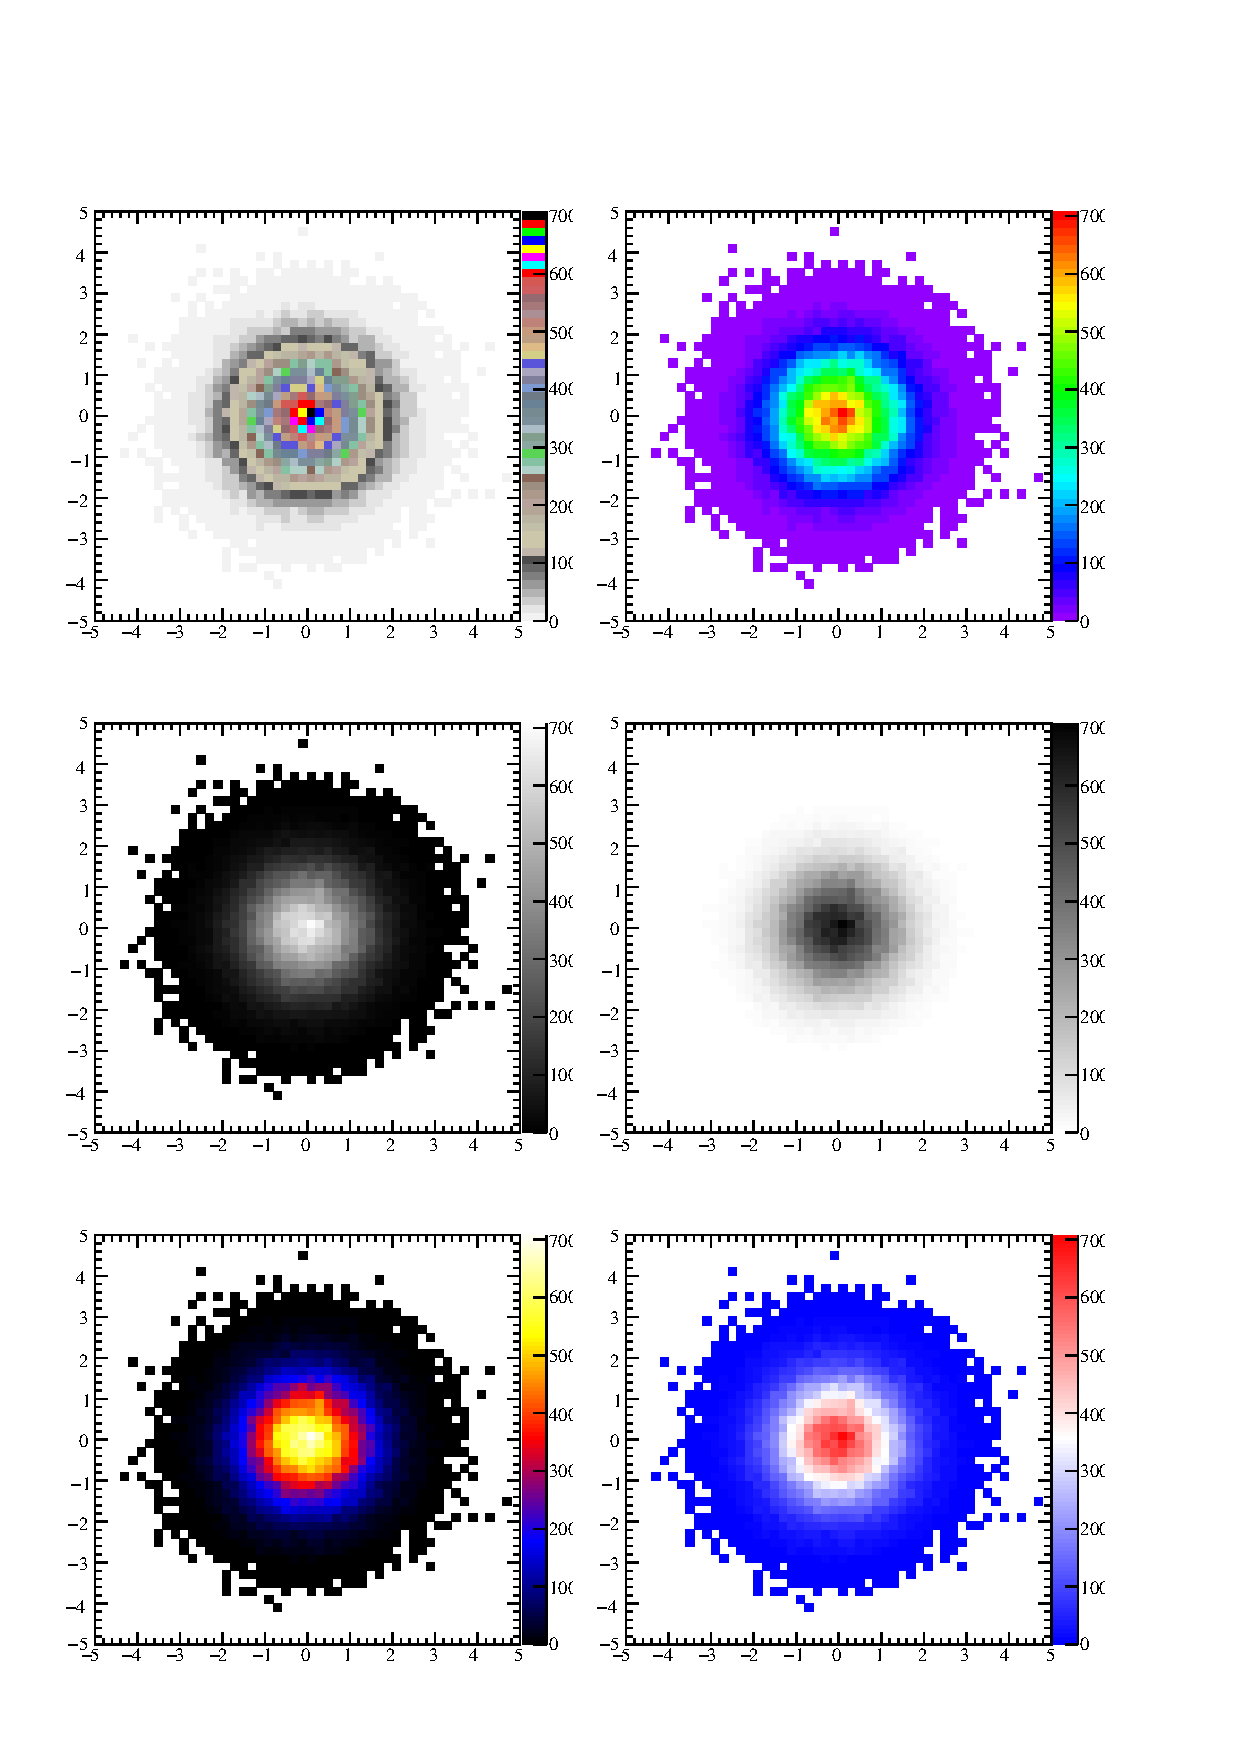
\includegraphics[width=12cm,clip]{fig/multi_palette.pdf}
  \caption{コード\ref{code:multi_palette}の出力結果}
  \label{fig:multi_palette_pdf}
\end{figure}

\subsection{塗りつぶしの色を変更する}

図\ref{fig:multi_palette_pdf}で様々なパレットを例示しました。既にお気付きの通り、値が0のビンはROOTは塗りつぶしません。そのため、空っぽのビンは全て白くなっています。図\ref{fig:multi_palette_pdf}の右上のように、パレットに白が含まれていない場合は、白いままのほうがヒストグラムの状態を把握するのに便利です。しかしパレット中に白が含まれている場合は、値が0なのか、他の値なのか判断できない場合が出てきます。そのような場合は、フレームの色を変更しましょう。

\begin{NoFloat}
\lstinputlisting[language=c++,caption=\texttt{frame\_fill\_color.C},label=code:frame_fill_color,numbers=left]{src/frame_fill_color.C}
\end{NoFloat}

コード\ref{code:frame_fill_color}は、フレームの背景色を変更する方法です。出力結果は図\ref{fig:frame_fill_color_pdf}に示します。

\begin{lstlisting}[language=C++]
  TPaletteAxis* palette 
    = (TPaletteAxis*)hist->GetListOfFunctions()->FindObject("palette"); 
\end{lstlisting}
この部分では、ヒストグラムから\texttt{TPaletteAxis}\footnote{図\ref{fig:frame_fill_color_pdf}の右端にあるグラデーション付き目盛りのことです。}のポインタを取得します。その直前の行で\texttt{gPad}を更新しないと\texttt{0}を返すので注意してください。
\begin{lstlisting}[language=C++]
  gPad->SetFrameFillColor(col); 
\end{lstlisting}
で、\texttt{gPad}の塗りつぶしの色を決定しています。この例では、最小値の色は黒になっています。

\begin{figure}
  \centering
  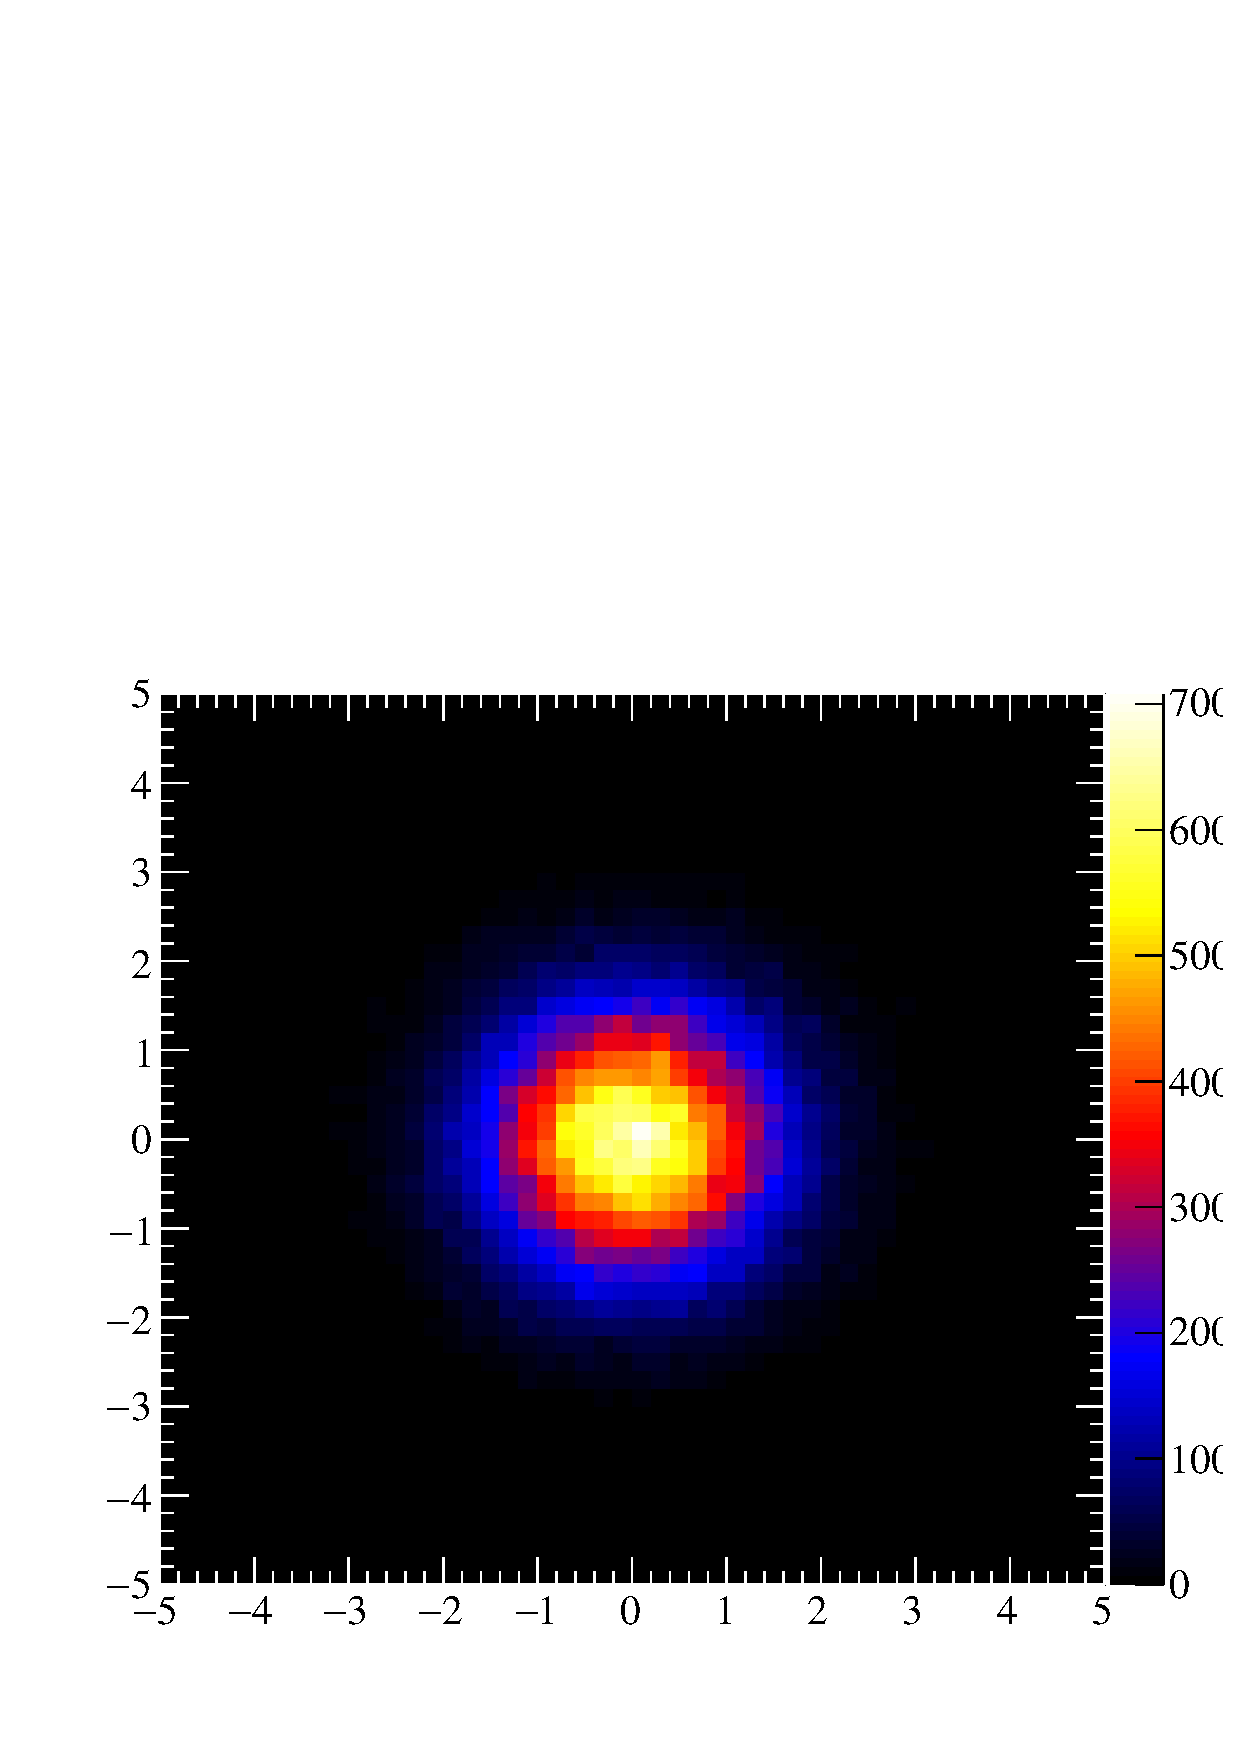
\includegraphics[width=8cm]{fig/frame_fill_color.pdf}
  \caption{コード\ref{code:frame_fill_color}の出力結果}
  \label{fig:frame_fill_color_pdf}
\end{figure}


\section{キャンバス関連}
\subsection{描画領域の大きさを指定する}
通常、新たなキャンバスを作成するときに大きさを指定する場合は、
\begin{lstlisting}[language=C++]
root [0] TCanvas* can = new TCanvas("can", "can", 100, 100)
\end{lstlisting}
のように第3、第4引数に横幅と高さを指定します。しかし予想外にも、図\ref{fig:100x100_png}に示すように、実はこの大きさは描画領域の大きさではありません。メニューバーは描画領域外周部まで含めた大きさなのです。したがって、実際に描画できる部分の大きさは、筆者の環境では$96\times72$ピクセルになってしまいます。図\ref{fig:100x100_v2_png}のように、描画領域を正確に$100\times100$ピクセルにしたい場合は、コード\ref{code:ExactSizeCanvas}のような関数を用意しましょう。

\begin{figure}
  \centering
  \subfigure[]{
    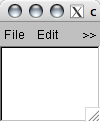
\includegraphics[width=3cm]{fig/100x100.png}
    \label{fig:100x100_png}
  }%
  \subfigure[]{%
    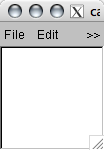
\includegraphics[width=3cm]{fig/100x100_v2.png}
    \label{fig:100x100_v2_png}
  }
  \caption{\texttt{TCanvas}の描画領域の違い。(a) $96\times72$ピクセル。(b) $100\times100$ピクセル。}
\end{figure}

\begin{NoFloat}
\lstinputlisting[language=c++,caption=\texttt{ExactSizeCanvas.C},label=code:ExactSizeCanvas,numbers=left]{src/ExactSizeCanvas.C}
\end{NoFloat}

次のように、\texttt{ExactSizeCanvas.C}をロードしてから、\texttt{ExactSizeCanvas}関数を\texttt{TCanvas}のコンストラクタのように使用すれば、描画領域が丁度$400\times400$ピクセルのキャンバスが得られます。
\begin{lstlisting}[language=C++]
root [0] .L ExactSizeCanvas.C
root [1] TCanvas* can = new ExactSizeCanvas("can", "can", 400, 400)
\end{lstlisting}
もし、得られた描画領域が$400\times400$でない場合は、お使いのコンピュータの画面の高さが$1000$ピクセル未満の可能性があります\footnote{画面が小さすぎるとROOTが勝手に判断し、\texttt{TCanvas}の大きさを自動調整するためです。}。\texttt{~/.rootrc}の
\begin{lstlisting}
Canvas.UseScreenFactor:     true
\end{lstlisting}
という行を
\begin{lstlisting}
Canvas.UseScreenFactor:     false
\end{lstlisting}
に変更するか、
\begin{lstlisting}[language=C++]
root [0] gStyle->SetScreenFactor(1.)
\end{lstlisting}
を実行して再度試してみてください。

またコンピュータの処理速度によっては、\texttt{TCanvas::SetWindowSize}の結果が反映されるまでに次の処理が開始される場合があります。例えば
\begin{lstlisting}[language=C++]
can->SaveAs("foo.png");
can->SaveAs("bar.png");
\end{lstlisting}
のように2回連続でPNG画像を保存させると、2つの画像のサイズがウインドウサイズ変更前と変更後になる場合があります。そのようなときは、
\begin{lstlisting}[language=C++]
gSystem->Sleep(100);
\end{lstlisting}
のような行を足すことで、処理待ちをさせることも可能です。

\section{グラフ関連}
\subsection{残差を表示する}

\begin{figure}
  \centering
  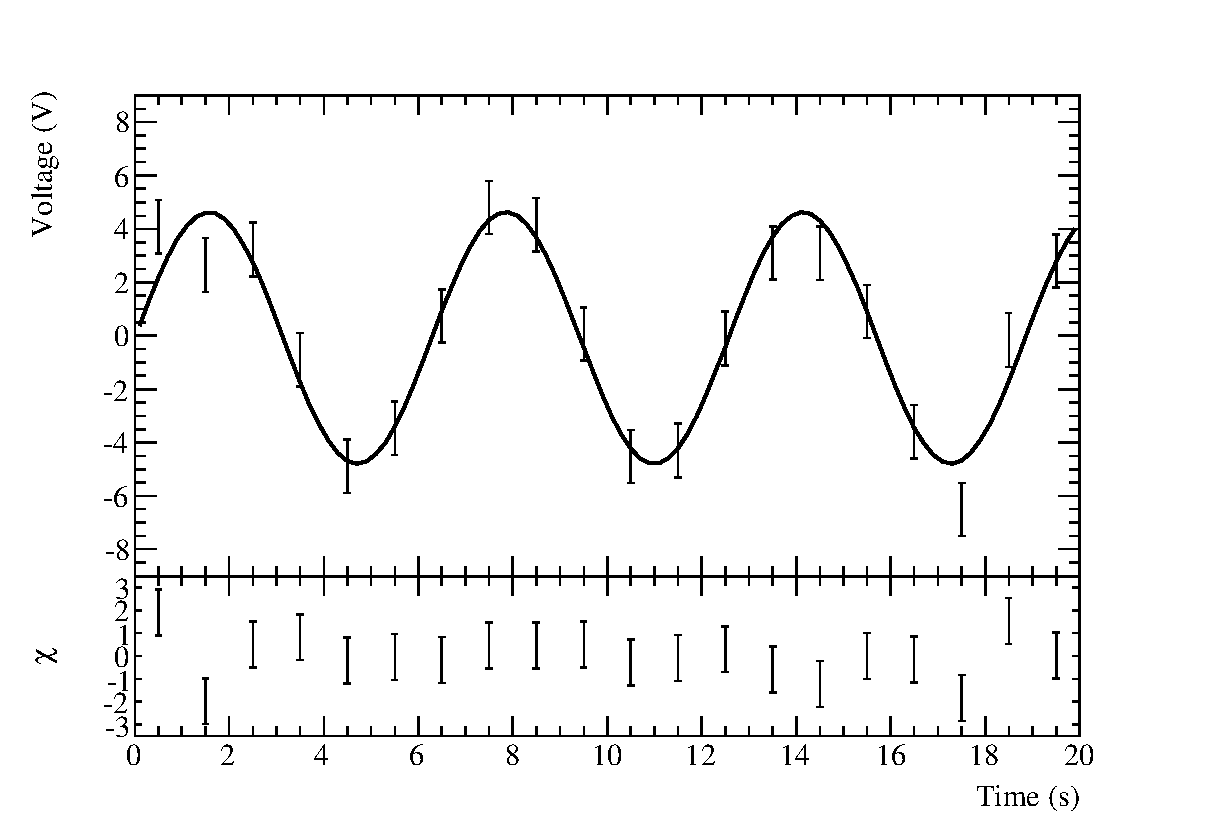
\includegraphics[width=12cm,clip]{fig/residual.eps}
  \caption{コード\ref{code:residual}の出力結果}
  \label{fig:residual_eps}
\end{figure}

\begin{NoFloat}
\lstinputlisting[language=c++,caption=\texttt{residual.C},label=code:residual,numbers=left]{src/residual.C}
\end{NoFloat}
